\documentclass{beamer}
\usepackage[brazil]{babel}
\usepackage[T1]{fontenc}
\usepackage[utf8]{inputenc}
\usepackage{url}
\usepackage{bibentry}
\usepackage{graphicx}
\usepackage[alf]{abntex2cite}

% \usetheme{Warsaw}
\usetheme{CambridgeUS}
\usecolortheme{dolphin}
\useoutertheme[footline=authortitle]{miniframes}
 
\begin{document}
 
\title[IFRN - CNAT]
      {Relatório Técnico de Desenvolvimento da Biblioteca Mirobot-Poti}
      \author[Mateus Oliveira Costa Bezerra]
             {Mateus Oliveira Costa Bezerra \\ Orientador: Prof. Me. Leonardo Ataide Minora}
  \institute{Instituto Ferderal de Educação, Ciência e Tecnologia do Rio Grande
    do Norte \\ Campus Natal-Central}
  \date{14 de fevereiro de 2017}

\begin{frame}
  \label{capa}
  \maketitle
\end{frame}

\begin{frame}
  \label{sumario}
  \frametitle{Sumário}
  \tableofcontents
  
\end{frame}

\begin{frame}
  \label{tangivel}
  \section{Introdução}
  \subsection{Programação Tangível}
  \frametitle{Programação Tangível: AlgoBlock}
       \begin{center}
         \begin{figure}
           
         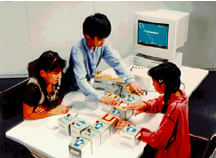
\includegraphics[width=8cm]{imagens/tangible.png}
          \caption{\tiny AlgoBlocs(1992) Suzuki e H. Kato}
         \end{figure}


     \end{center}
\end{frame}


 
\begin{frame}
  \frametitle{Programação Tangível: Logo}
  \begin{center}
    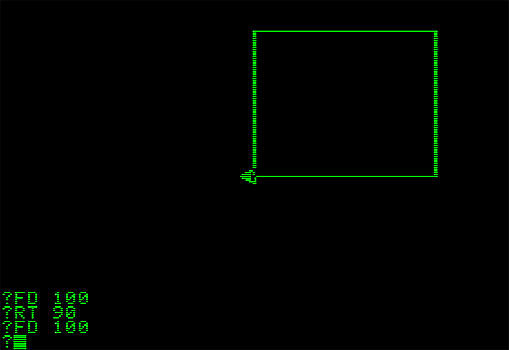
\includegraphics[width=8cm]{imagens/logo1.jpg}
    \end{center}
\end{frame}

\begin{frame}
  \frametitle{Programação Tangível: Logo}
  \begin{center}
    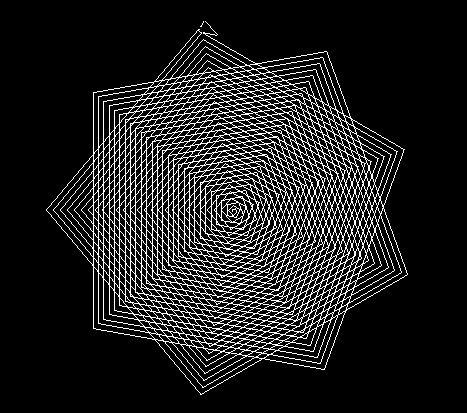
\includegraphics[width=8cm]{imagens/logo2.png}
  \end{center}
\end{frame}


\begin{frame}
  \begin{block}{Conceito}
    \begin{itemize}
    \item Programação Tangível se a refere a atividade de arranjar os blocos para \textbf{construir}(no sentido oposto de ``escrever'') programas de computador. ~\cite{McNerney2000}
    \end{itemize}
  \end{block}
  
  \begin{block}{Caracteristicas}
    \begin{itemize}
    \item É a mistura entre a maleabilidade da programação e a interatividade dos blocos.~\cite{McNerney2000}
    \item Diferente de manipular objetos virtuais, você manipula objetos reais para se comunicar com o computador.~\cite{McNerney2000}
    \end{itemize}
    \end{block}  
\end{frame}

\begin{frame}
  \label{mirobot}
  \subsection{Mirobot}
  \frametitle{Mirobot}
  
  \begin{center}
    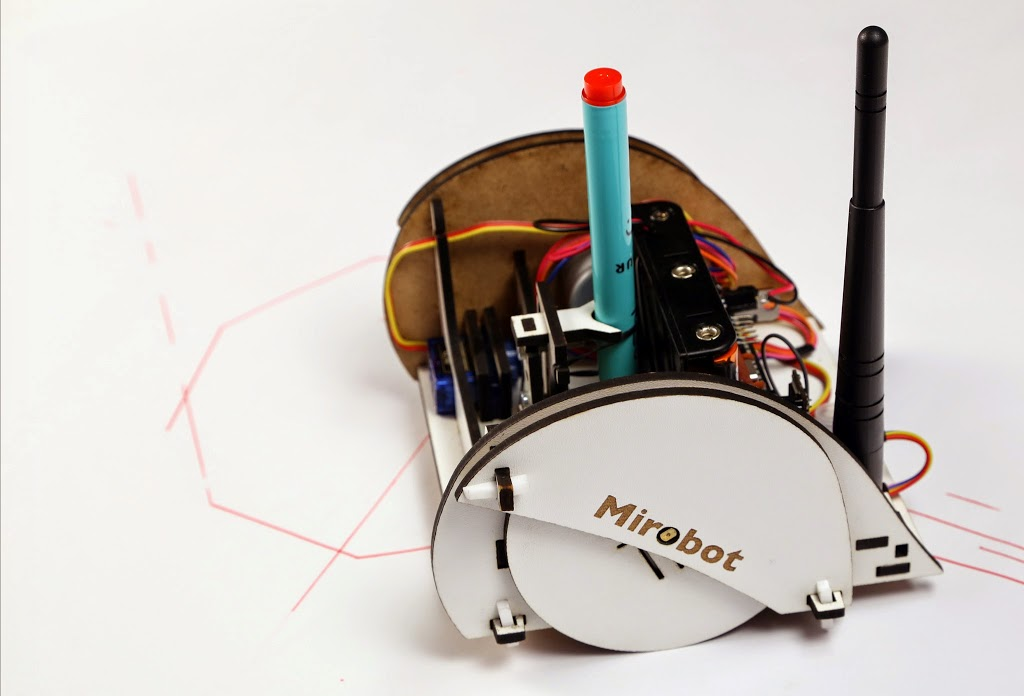
\includegraphics[width=10cm]{imagens/mirobot.jpg}
  \end{center}

\end{frame}

\begin{frame}
  \label{Potigol}
  \subsection{Potigol}
  \frametitle{Potigol}
  \begin{block}{História ~\cite{HellenLemos}}
        \begin{itemize}
    \item Projeto iniciado no ano de 2011 no IFRN - CNAT.
    \item Prof. Leonardo Reis Lucena.
     \item Aplicação nos cursos técnicos e superiores.  
        \end{itemize}

  \end{block}
  
        \begin{block}{Características}
          \begin{itemize}
          \item Sintaxe em \textbf{português}.
          \item Suporte multiparadigma.
          \item Planejada para ser usada por alunos iniciantes.
          \end{itemize}
        \end{block}
\end{frame}

\begin{frame}
  \section{Objetivo Geral do Trabalho}
  \frametitle{Objetivo Geral do Trabalho}
  \begin{center}
    Implementar uma biblioteca que permita programar na linguagem Potigol comportamentos de um robô Mirobot.
  \end{center}
\end{frame}
\begin{frame}
  \section{Desenvolvimento da Biblioteca}
  \subsection{Protocolo do Mirobot}
  \label{protocolo}
  \frametitle{Protocolo do Mirobot}
\end{frame}

\begin{frame}
  \subsection{Métodos do Mirobot}
  \label{metodos}
  \frametitle{Métodos do Mirobot}
\end{frame}

\begin{frame}
  \subsection{Implementação dos Métodos do Mirobot}
  \label{implementacao}
  \frametitle{Implementação dos Métodos do Mirobot}
\end{frame}

\begin{frame}
  \subsection{Exemplo de Uso da Biblioteca Mirobot-Poti}
  \label{exemplo}
  \frametitle{Exemplo de Uso da Biblioteca Mirobot-Poti}
\end{frame}

\begin{frame}
  \label{consideracoes}
  \section{Considerações Finais}
  \frametitle{Considerações Finais}
\end{frame}

\begin{frame}
  \label{referencias}
  \section{Referências}
  \frametitle{Referências}
%\bibliographystyle{amsalpha}
% \bibliographystyle{apalike}
\bibliographystyle{abntex2-alf}
  \bibliography{Referencias}
\end{frame}

\end{document}
